\chapter{Evaluations}
\label{cha:eval}
{\colorGreen
To evaluate the effectiveness of our system, we conduct two sets of evaluations:
\begin{itemize}
    \item Performance evaluation of RepoGraph, the frontend context retrieval algorithm, across models of different sizes and specialties. This assesses the consistency, robustness, and portability of the algorithm when under resource constraints and/or the backend model's reasoning capability is limited. We additionally evaluate the impact of CacheBlend's KV cache reuse on output quality.
    \item Latency evaluation for CacheBlend, the backend KV cache reuse module, specifically under agentic workloads. This differentiates from the original work's evaluations with QA and text-based RAG workloads, and is critical for understanding the applicability of the caching scheme in agentic settings.
\end{itemize}}


\section{Performance Evaluation for Context Retrieval}
\label{sec:ch1_eval}

\subsection{Setup}
The evaluation of RepoGraph largely follows the methods of the original paper, where it is utilized as a plug-in component on top of an existing agentic framework. For the purpose of our study, we chose the Agentless procedural framework. The advantage of integrating a procedural framework in lieu of a traditional agent is simplicity and comprehensibility. In the case of Agentless, it deploys a three-phase process of localization, repair, and patch validation \cite{xia2024agentlessdemystifyingllmbasedsoftware}. Intermediate results are transparent between each step, where empty or error responses are immediately identifiable. This allows for finding bottlenecks and comparing performance against various models on step granularity. 

Our goal is to verify the consistency of the integrated agent's performance across LLM backends of different parameter sizes and architectures. For this purpose, we conducted experiments for RepoGraph + Agentless using a set of models with different configurations (for details see \hyperref[sec:ch1_eval_model]{Models}). 
\subsubsection{Metric}
% resolve rate as in RepoGraph original paper, patch application rate optional. 
We will continue the usage of resolve rate following the original work as our primary evaluation metric. An instance is considered resolved if: 1. The generated patch is successfully applied to the repository, and 2. The postfix code passes all test suites. 

This metric provides a direct measure of end-to-end task success, capturing not only whether a patch is syntactically correct but also whether it integrates cleanly into the repository and satisfies the intended functionality. Compared to intermediate measures such as code similarity or partial compilation success, the resolve rate reflects the practical utility of the generated patches and therefore serves as a good indicator of real-world performance.


% The resolve rate represents the percentage of issues successfully resolved across all data points. An issue is considered
% resolved if the submitted patch passes all test scripts. To assess the patch application rate, we attempt
% to apply the generated patches to the repository using the patch program, counting only successful
% applications toward this metric
\subsubsection{Datasets}

For a comprehensive yet time and cost efficient evaluation, we run our experiments in SWE-bench Verified-mini \cite{MariusHobbhahn2025swe-bench-verified-mini}, which is a subset of SWE-bench Verified\cite{chowdhury2024swebenchverified} that is selected via k-means clustering and linear programming, such that the marginal distributions of important scores are preserved. This is a smaller dataset than SWE-bench Lite\cite{yang2024sweagent}, yet high-quality and well-specified, and is capable of reflecting an agent's performance across a spectrum of task difficulties.
\subsubsection{Models}
\label{sec:ch1_eval_model}
% GPT4/4o, Claude Sonnet 3.5, Gemini, Qwen3-coder, Deepseek, etc.
To ensure consistency, robustness, and portability of RepoGraph as our repository-aware context retrieval algorithm, it is important to evaluate it against multiple model backends of varying architectures and parameter scales. Different models exhibit distinct behaviors in terms of tokenization, embedding spaces, and context utilization. A retrieval method that aligns well with one tokenizer or attention mechanism may under-perform when paired with another, which makes cross-model testing critical for avoiding over-specialization.

In addition, models differ in how they exploit the retrieved context. More powerful models may compensate for imperfect retrieval given stronger reasoning and synthesis capabilities, whereas smaller models are more sensitive to accuracy and relevance of the retrieved context. Thus, evaluating across a spectrum of models provides insight into how much of RepoGraph’s performance benefits stem from the context retrieval strategy itself. This also allows us to characterize situations where retrieval quality is most impactful, particularly in cost-constrained settings where smaller models are attractive.

Finally, cross-backend evaluation provides practical benefits for deployment. Since real-world systems often migrate between providers (e.g., OpenAI, Anthropic, Mistral), retrieval algorithms must remain portable to ensure stable performance under backend substitution. For our experiments, we therefore consider a representative set of both proprietary and open-source models, including \textbf{GPT-4o, o4-mini, Claude 3.5 Sonnet, and Devstral Small}, covering a range of architectures, parameter counts, and costs.

\subsection{Results}

\begin{figure}[ht]
\centering
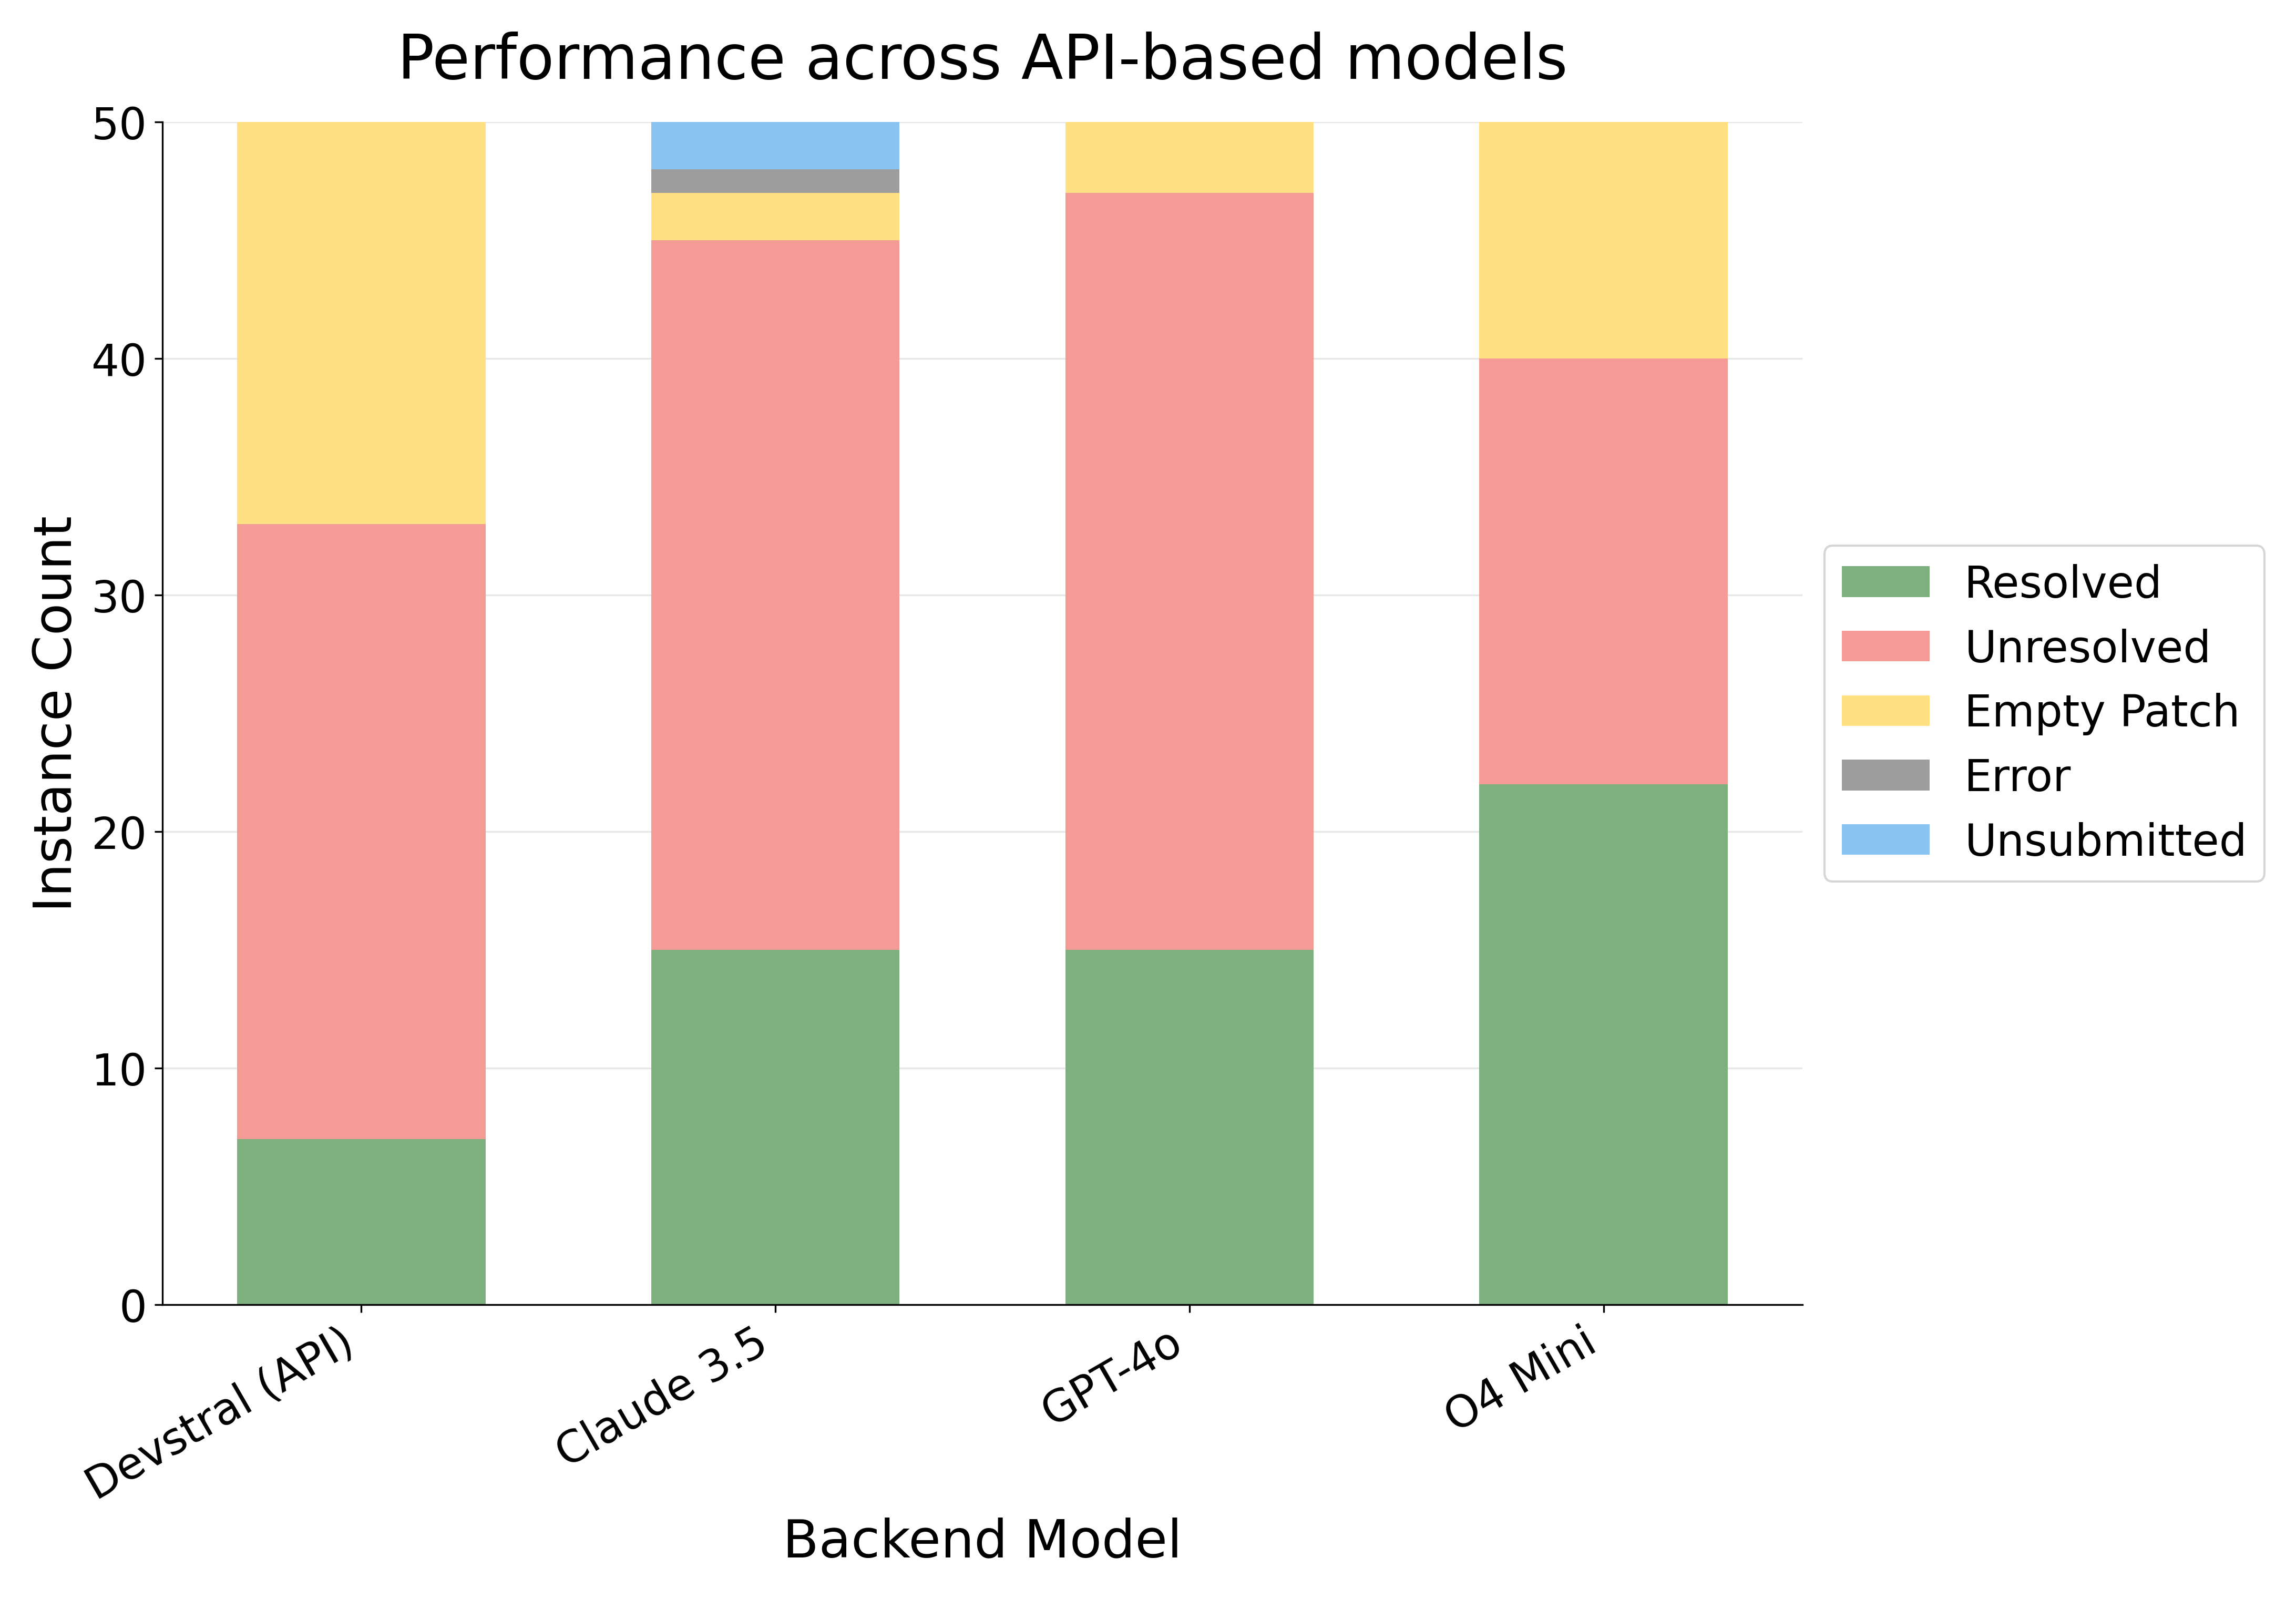
\includegraphics[width=0.75\linewidth]{graphs/v0_plots/visualized_eval_mini_results_all.png}
\vspace{-0.2in}
  \caption{\small Full results distributions for SWE-bench Verified-mini evaluation runs across different models.}
 \label{fig:repograph_api_perf}
 \vspace{-0.15in}
\end{figure}

To further assess whether CacheBlend's KV cache reuse affects output quality, we run an additional evaluation using Devstral Small hosted on vLLM with LMCache (CacheBlend enabled) on the same SWE-bench Verified-mini dataset. We compare different blending granularities against the baseline (no blending) to verify that position-independent cache reuse does not degrade patch quality.

\begin{figure}[ht]
\centering
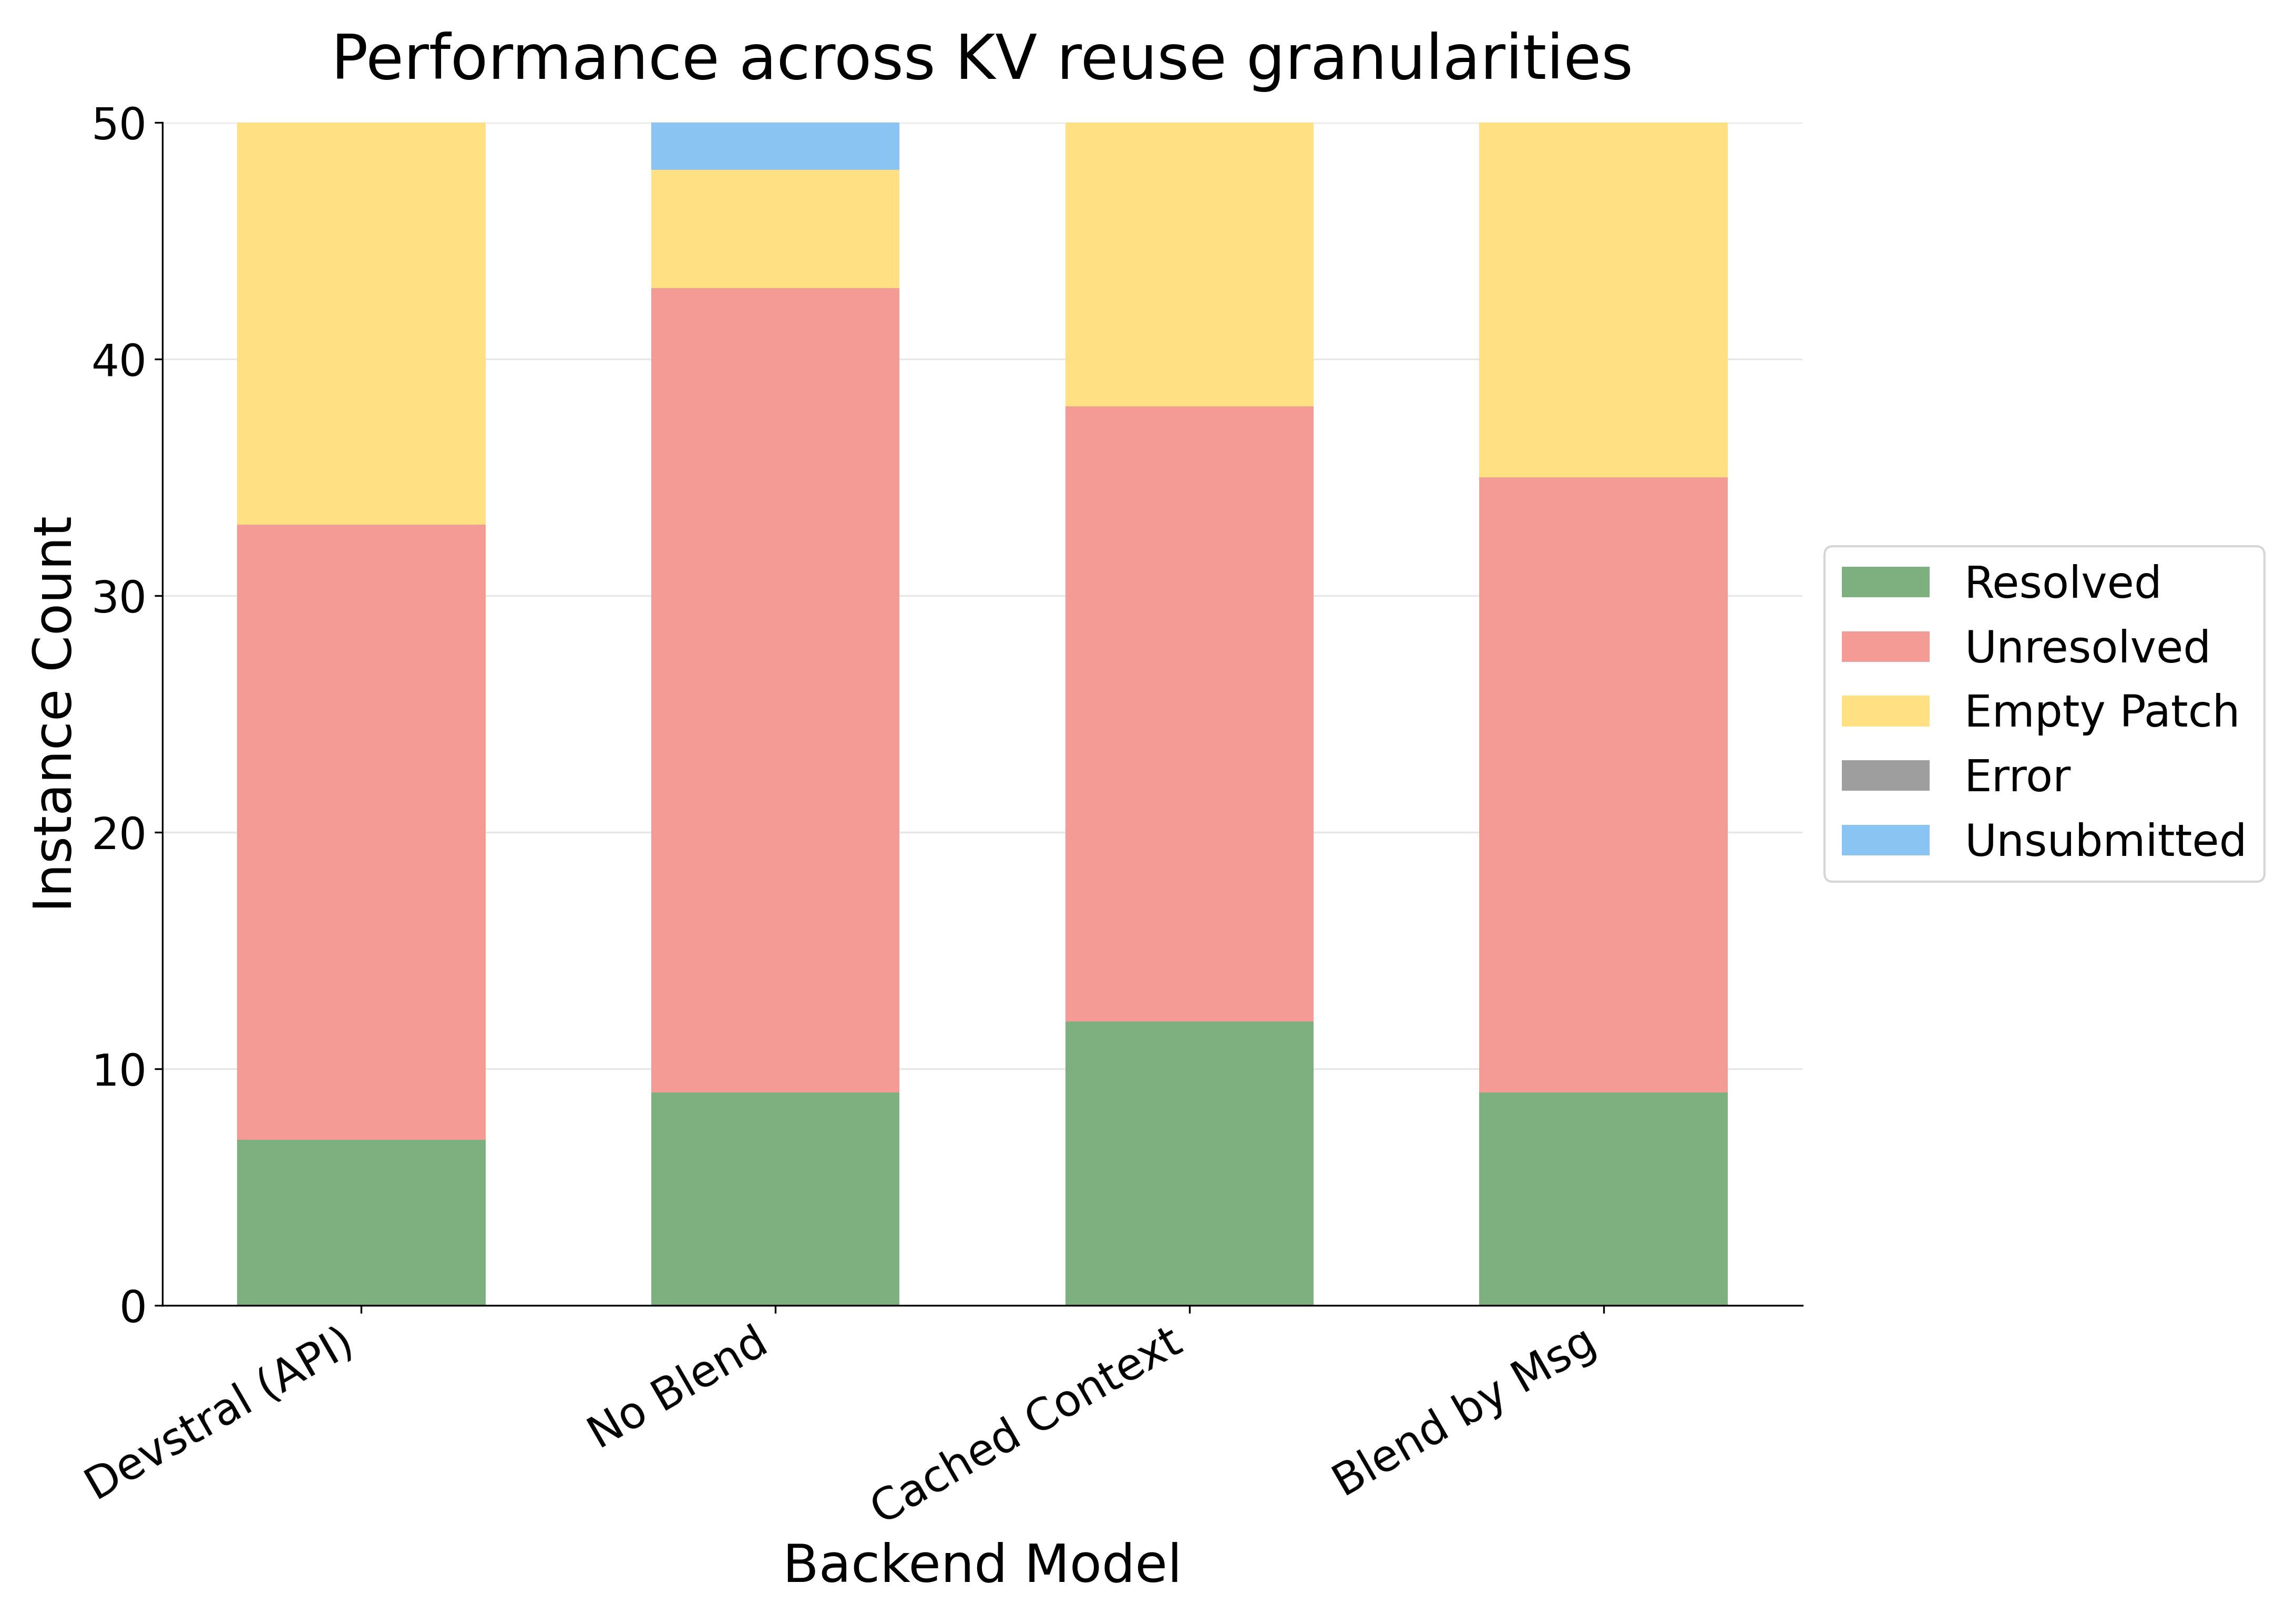
\includegraphics[width=0.75\linewidth]{graphs/v0_plots/visualized_eval_mini_results_lmcache.png}
\vspace{-0.2in}
  \caption{\small Results distributions for SWE-bench Verified-mini evaluation runs across different blending methods, served model is Devstral Small.}
 \label{fig:e2e_blended_perf}
 \vspace{-0.15in}
\end{figure}